\documentclass[tikz]{standalone}
\usepackage{tikz}
\usetikzlibrary{positioning, graphs}
\usetikzlibrary{graphs.standard}
\begin{document}
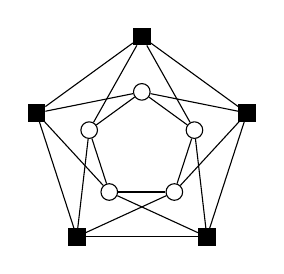
\begin{tikzpicture}
    [circle_node/.style={circle, draw, inner sep = 0, minimum size = 0.6em},
     rectangle_node/.style={rectangle, draw, inner sep = 0, minimum size = 0.6em, fill=black}]

    \graph[clockwise, radius=4em, phase=18, empty nodes, nodes=rectangle_node]{subgraph C_n[n = 5, name = A]};
    \graph[clockwise, radius=2em, phase=18, empty nodes, nodes=circle_node]{subgraph C_n[n = 5, name = B]};

    \foreach \i [evaluate={\j=int(mod(\i,5)+1)}] in {1,...,5}{
		\draw (A \i) -- (B \j);
		\draw (A \j) -- (B \i);
    }
\end{tikzpicture}
\end{document}